\chapter{Additional Graphs and Full Statistical Analysis Tables}


\begin{table}[htp]
\caption{duration \& quantity fixed effects}
\begin{center}
\begin{tabular}{|l|c|c|c|}
\hline
{\bf Predictors}	&	{\bf Estimates}	&	{\bf Confidence Interval}	&	{\bf p}	\\
\hline
\hline
(Intercept)	&	0.27	&	0.23 – 0.30	&	<0.001***	\\
Q2	&	-0.04	&	-0.06 – -0.02	&	<0.001***	\\
Q3	&	-0.03	&	-0.06 – -0.00	&	0.048*	\\
off-ictus &	-0.05	&	-0.08 – -0.02	&	0.004*	\\
Q2 * off-ictus	&	0.02	&	-0.03 – 0.06	&	0.54	\\

Q3 *off-ictus	&	-0.02	&	-0.07 – 0.03	&	0.44	\\
\hline
\end{tabular}
\end{center}
\label{qdurfixed}
\end{table}%
%%%%%%%%%%%%%%%%%%%%%%%%%%%%

\begin{table}[htp]
\caption{dquantity-duration random effects}
\begin{center}
\begin{tabular}{|l|c|c|c|}
\hline
{\bf Random Effects}	&		&		&		\\
\hline
{\bf Predictors}	&	{\bf Estimates} & & \\
\hline
$σ2$	&	0.0012	&		&		\\
τ00 word	&	0.0034	&		&		\\
τ00 song	&	0.0022	&		&		\\
τ00 performer	&	0.0001	&		&		\\
ICC	&	0.8227	&		&		\\
\hline
\hline
N song	&	9	&		&		\\
N word	&	298	&		&		\\
N performer	&	3	&		&		\\
Observations	&	367	&		&		\\
Marginal R2 / Conditional R2	&	0.071 / 0.835	&		&		\\
\hline
\end{tabular}
\end{center}
\label{qdurrandoms}
\end{table}%

%%%%%%%%%%

\begin{table}[htb]
\caption{model comparison, duration predicting quantity \& ictus}
\centering
\begin{tabular}{|ccccccccc|}
\hline
      & npar   &  AIC   &  BIC & logLik & deviance  & Chisq & Df & Pr(>Chisq)    \\
      \hline
null  &  5 &-914.74 &-895.21 &462.37  &-924.74        &&& \\                 
design  &  10 &-949.20 &-910.15 &484.60 & -969.20 & 44.464  &5  &1.865e-08 *** \\
\hline

\end{tabular}
\label{qcomp}
\end{table}%
 \footnote{Signif. codes:   ‘***’ 0.001 ‘**’ 0.01 ‘*’ 0.05 }

%%%%%%%


\begin{table}[htp]
\caption{anova of model comparison: duration dependent stressed ictus}
\begin{center}
\centering
\begin{tabular}{|ccccccccc|}
\hline
      & npar   &  AIC   &  BIC & logLik & deviance  & Chisq & Df & Pr(>Chisq)    \\
\hline
null &   5& -1747.0 &-1724.4  &878.5 & -1757.0         && \\       
\hline         
design &   10& -1966.8& -1921.6  &993.4  &-1986.8 & 229.81&  5 & < 2.2e-16 ***\\
\hline

\end{tabular}
\end{center}
\label{durstrickmdls}
\end{table}%

%
%\begin{equation*}
%
%des_null_md: euclid ~ (1 | segment) + (1 | song) + (1 | performer) \\
%desmd: euclid ~ stressed + ictus + stressed * ictus + (1 | segment) + (1 | song) + (1 | performer) \\
%\end{equation*}



\begin{table}[htp]
\caption{anova of design and null lmer models for euclidean distance, stress and ictus }
\begin{center}
\centering
\begin{tabular}{|ccccccccc|}

\hline
     &       npar  &  AIC   & BIC  & logLik & deviance  & Chisq & Df & Pr(>Chisq) \\
     \hline
null  &  5 & 5347.3 & 5367.3 & -2668.7  & 5337.3             \\        
design    &      8 & 5348.7& 5380.7 &-2666.4  & 5332.7 & 4.5855 & 3   &  0.2048 \\
\hline
\end{tabular}
\end{center}
\label{aoveuc}
\end{table}%


\begin{table}[htp]
\caption{duration dependent variable lmer}
\begin{center}
\begin{tabular}{|l|c|c|c|}
\hline
Predictors	&	Estimates	&	Confidence Intervals	&	p	\\
\hline
(Intercept)	&	0.22	&	0.18 – 0.25	&	<0.001***	\\
off-ictus	&	-0.03	&	-0.05 – -0.00	&	0.017**	\\
stressed	&	0.05	&	0.03 – 0.07	&	<0.001***	\\
Q2&	-0.05	&	-0.06 – -0.04	&	<0.001***	\\
off-ictus* stressed	&	-0.01	&	-0.04 – 0.02	&	0.467	\\
off-ictus* Q2	&	0.01	&	-0.01 – 0.03	&	0.332	\\
\hline
\end{tabular}
\end{center}
\label{durlmer}
\end{table}%
%%%%%%%%%%%%%

\begin{table}[htp]
\caption{random effects duration-stress-ictus model}
\begin{center}
\begin{tabular}{|l|c|}
\hline

{\bf Random Effects }	&	Confidence Intervals	\\
\hline
Predictors & Estimates \\
σ2	&	0.0026		\\
τ00 word	&	0.0004		\\
τ00 song	&	0.0018			\\
τ00 performer	&	0.0001		\\
ICC	&	0.4761		\\
\hline
N word	&	315			\\
N song	&	9			\\
N performer	&	3		\\
Observations	&	676		\\
Marginal R2 / Conditional R2	&	0.190 / 0.576	\\
\hline
\end{tabular}
\end{center}
\label{durlmerrando}
\end{table}%


%%%space
%%%%%%%%%%%

\begin{table}[htp]
\caption{euclidean distance dependent fixed effects}
\begin{center}
\begin{tabular}{|l|c|c|c|}
\hline							
Predictors	&	Estimates	&	Confidence Interval	&	p	\\
(Intercept)	&	351.9	&	207.53 – 496.26	&	<0.001***	\\
stressed 	&	48.7	&	-48.46 – 145.87	&	0.325	\\
off-ictus	&	80.8	&	-14.93 – 176.52	&	0.098	\\
stressed*off-ictus	&		&		&		\\
\hline							
\end{tabular}
\end{center}
\label{euclmer}
\end{table}%



\begin{table}[htp]
\caption{random effects of euclidean distance and stress-ictus lmer}
\begin{center}
\begin{tabular}{|l|c|}
\hline							
Random Effects	&						\\
\hline
σ2	&	32259.12					\\
τ00 segment	&	4058.78					\\
τ00 song	&	5512.35					\\
τ00 performer	&	5432.4					\\
ICC	&	0.32					\\
\hline
N segment	&	11					\\
N song	&	9					\\
N performer	&	3					\\
Observations	&	401					\\
Marginal R2 / Conditional R2	&	0.008 / 0.323					\\						
\hline							
\hline							
\end{tabular}
\end{center}
\label{randolmereuc}
\end{table}%


\begin{figure}[htb]
\centering
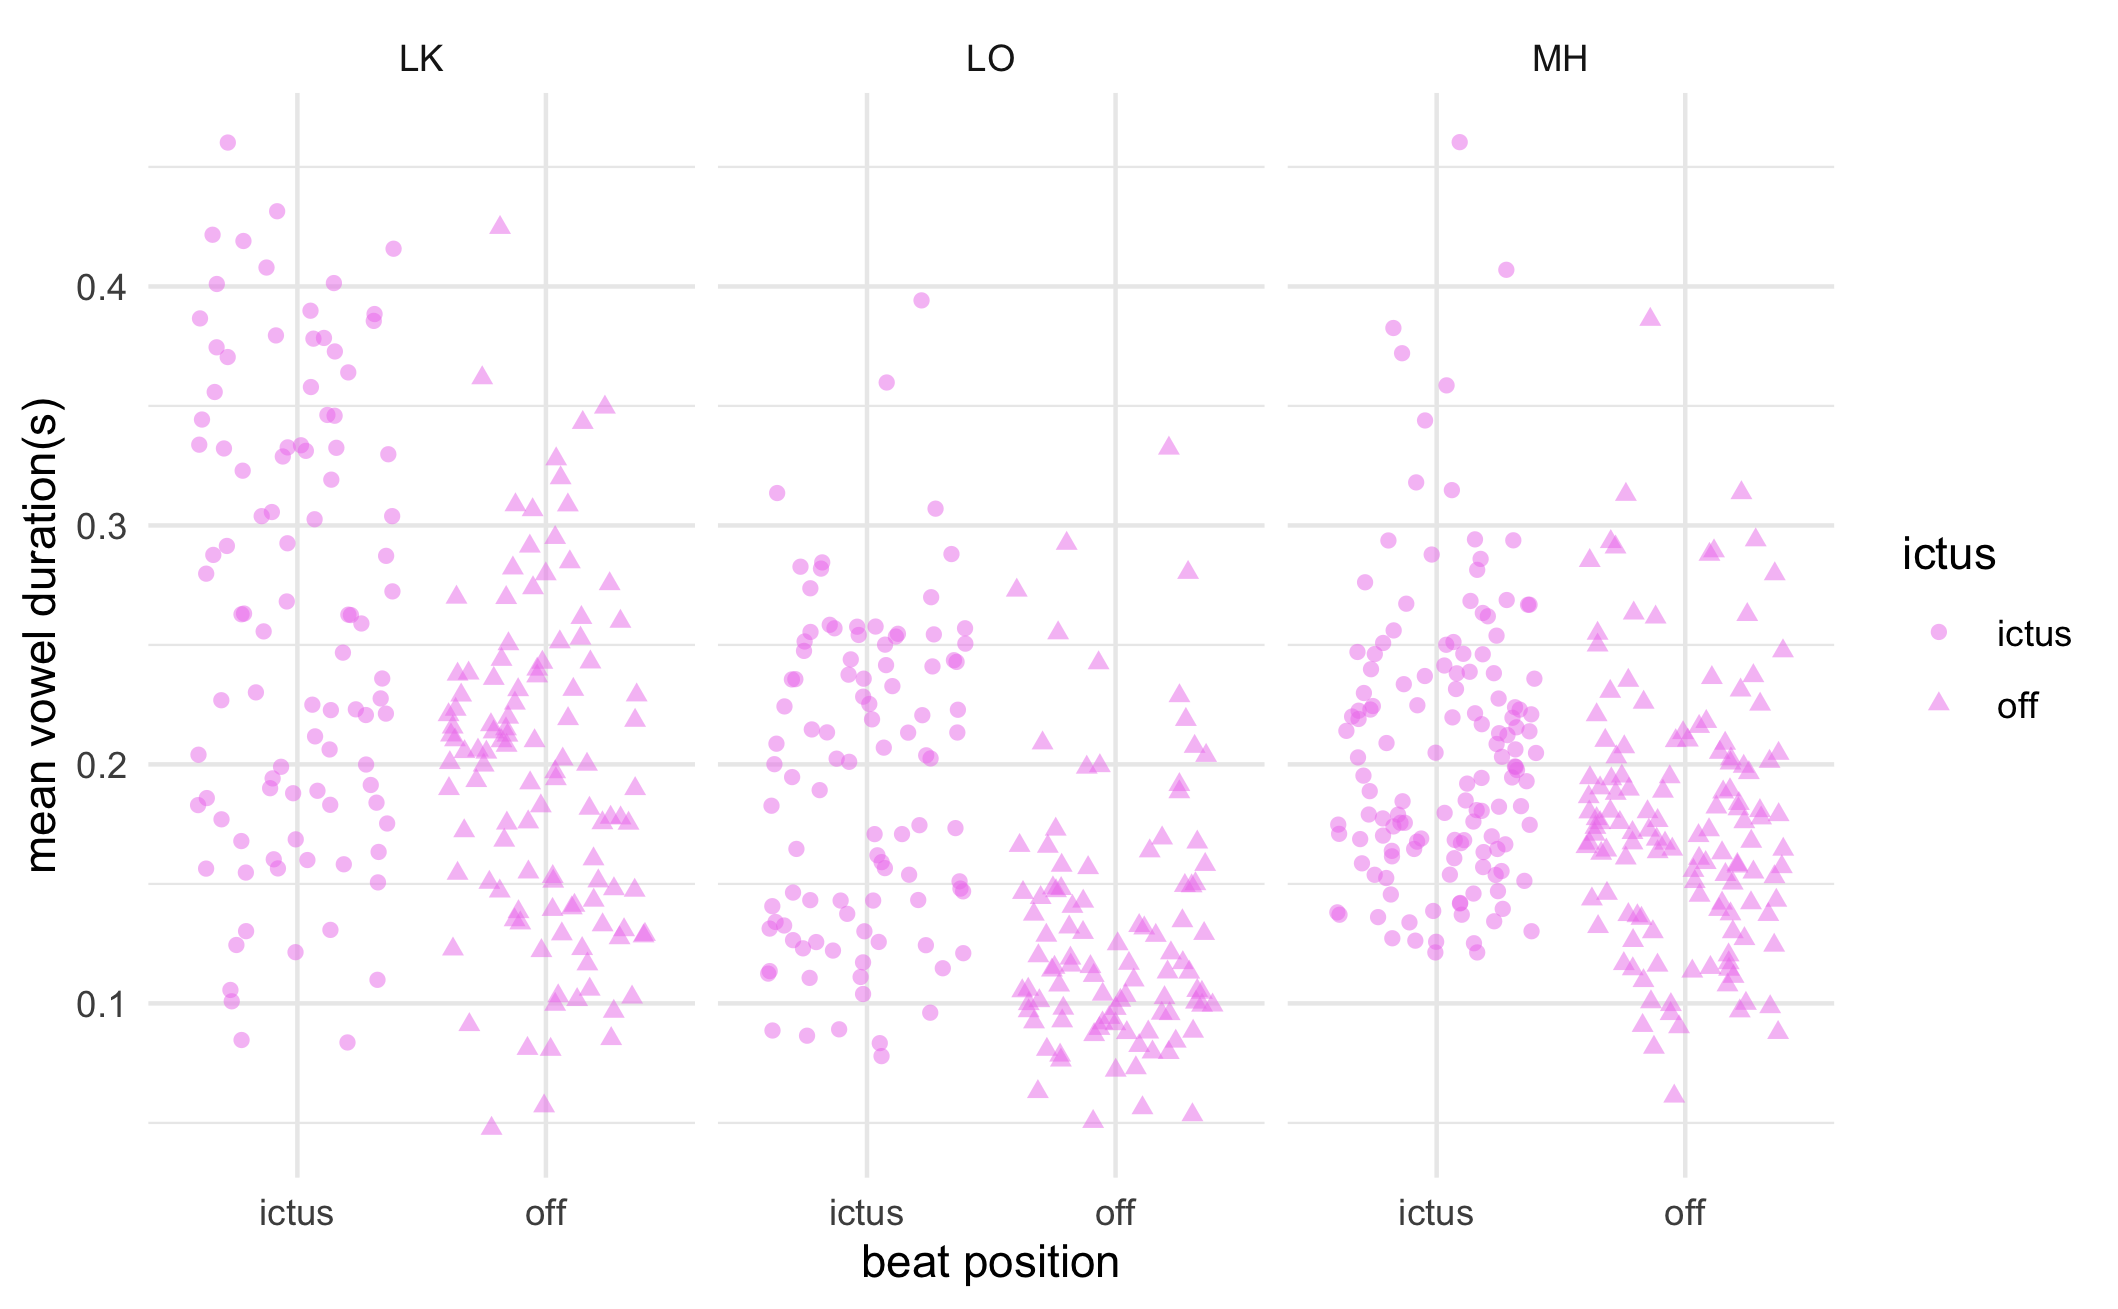
\includegraphics[width=\textwidth]{/Users/sarah/Git/regilaul_project/manuscript/results/perf_ick_dur.png}

\caption{vowel durations on and off the beat in each performer}
\label{perfbeats}


\end{figure}

%%%%%%%%%
\begin{figure}[htb]
\centering
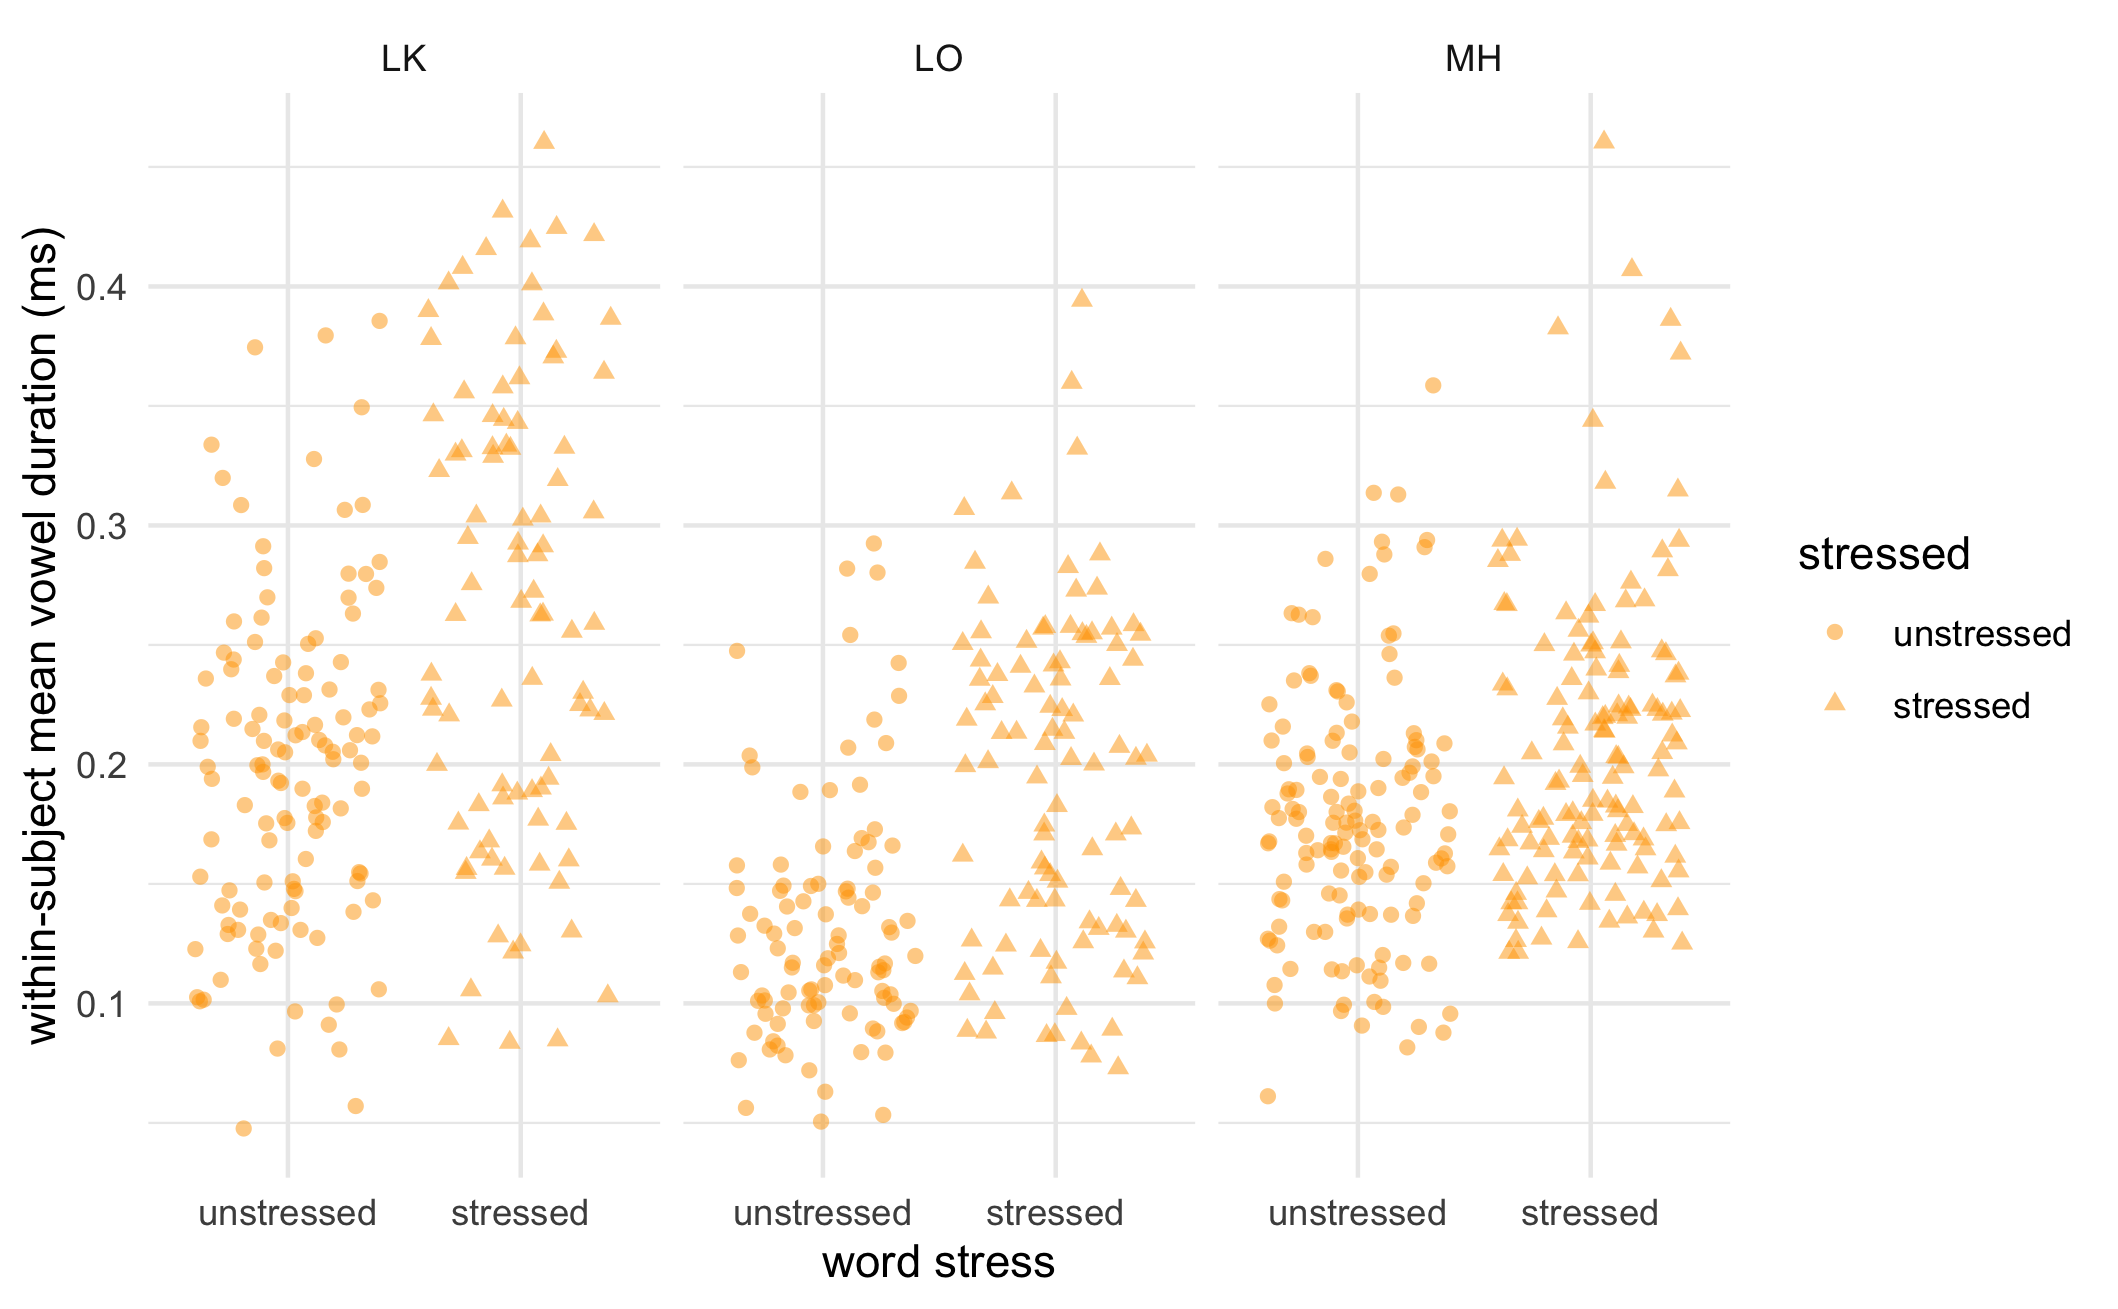
\includegraphics[width=\textwidth]{/Users/sarah/Git/regilaul_project/manuscript/results/perf_str_dur.png}

\caption{vowel durations of word-stress in each performer}
\label{perfstr}
\end{figure}


%%%%%%%%%%%%%


\begin{figure}[htb]
\centering
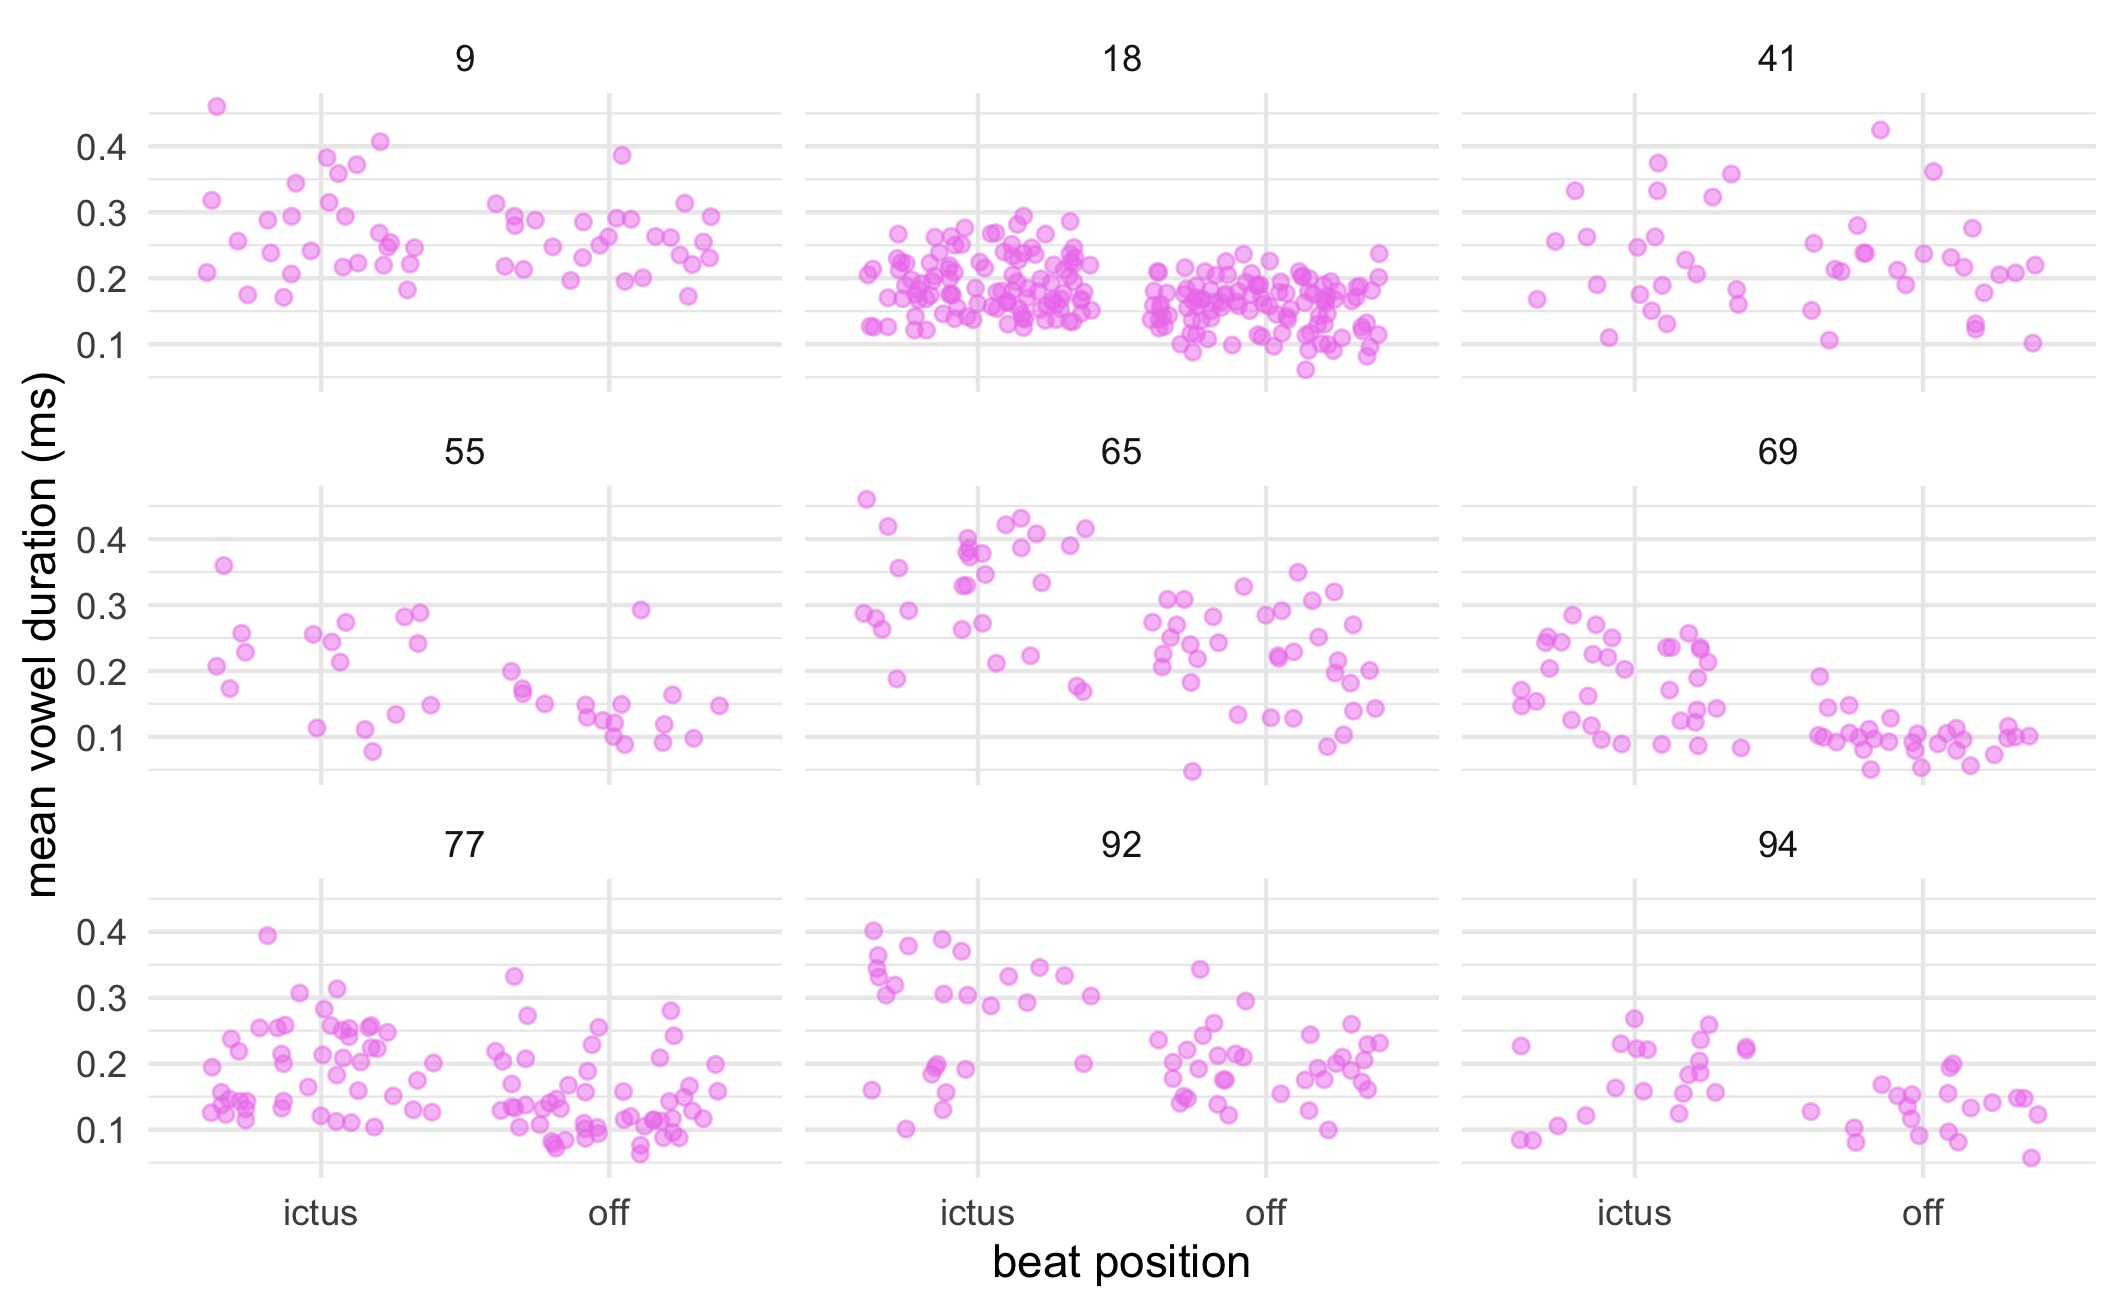
\includegraphics[width=\textwidth]{/Users/sarah/Git/regilaul_project/manuscript/results/song_icK_dur.png}

\caption{vowel durations on and off the beat by song}
\label{sonicdur}

\end{figure}



%%%%%%%%%%%


\begin{figure}[htb]
\centering
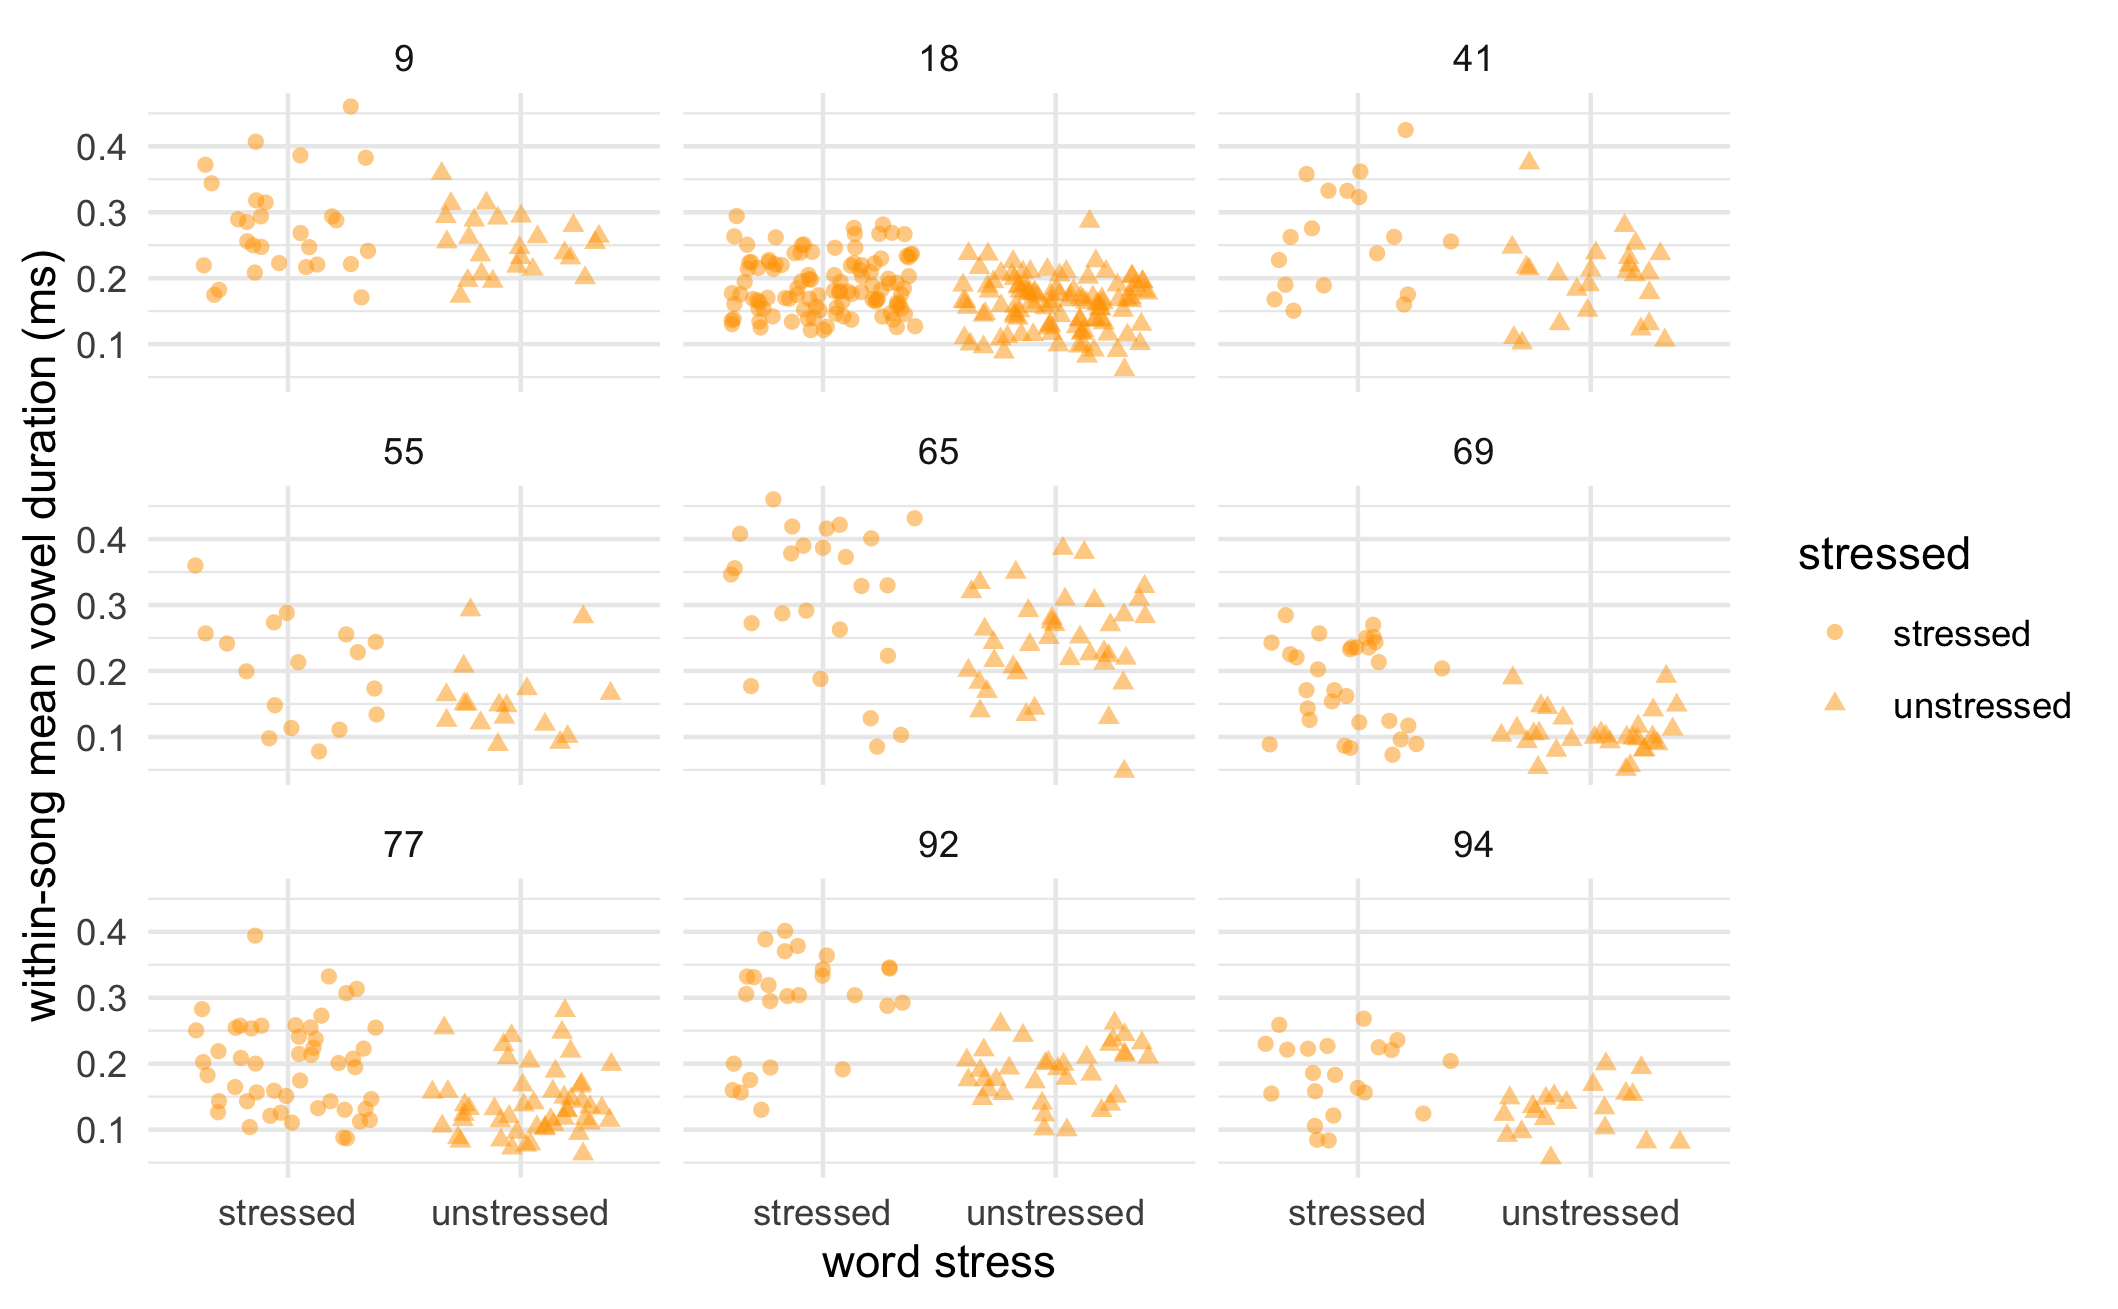
\includegraphics[width=\textwidth]{/Users/sarah/Git/regilaul_project/manuscript/results/song_str_dur.png}

\caption{within-song vowel durations in each word-stress position}
\label{sonstrdur}

\end{figure}



\begin{figure}[htb]
\centering
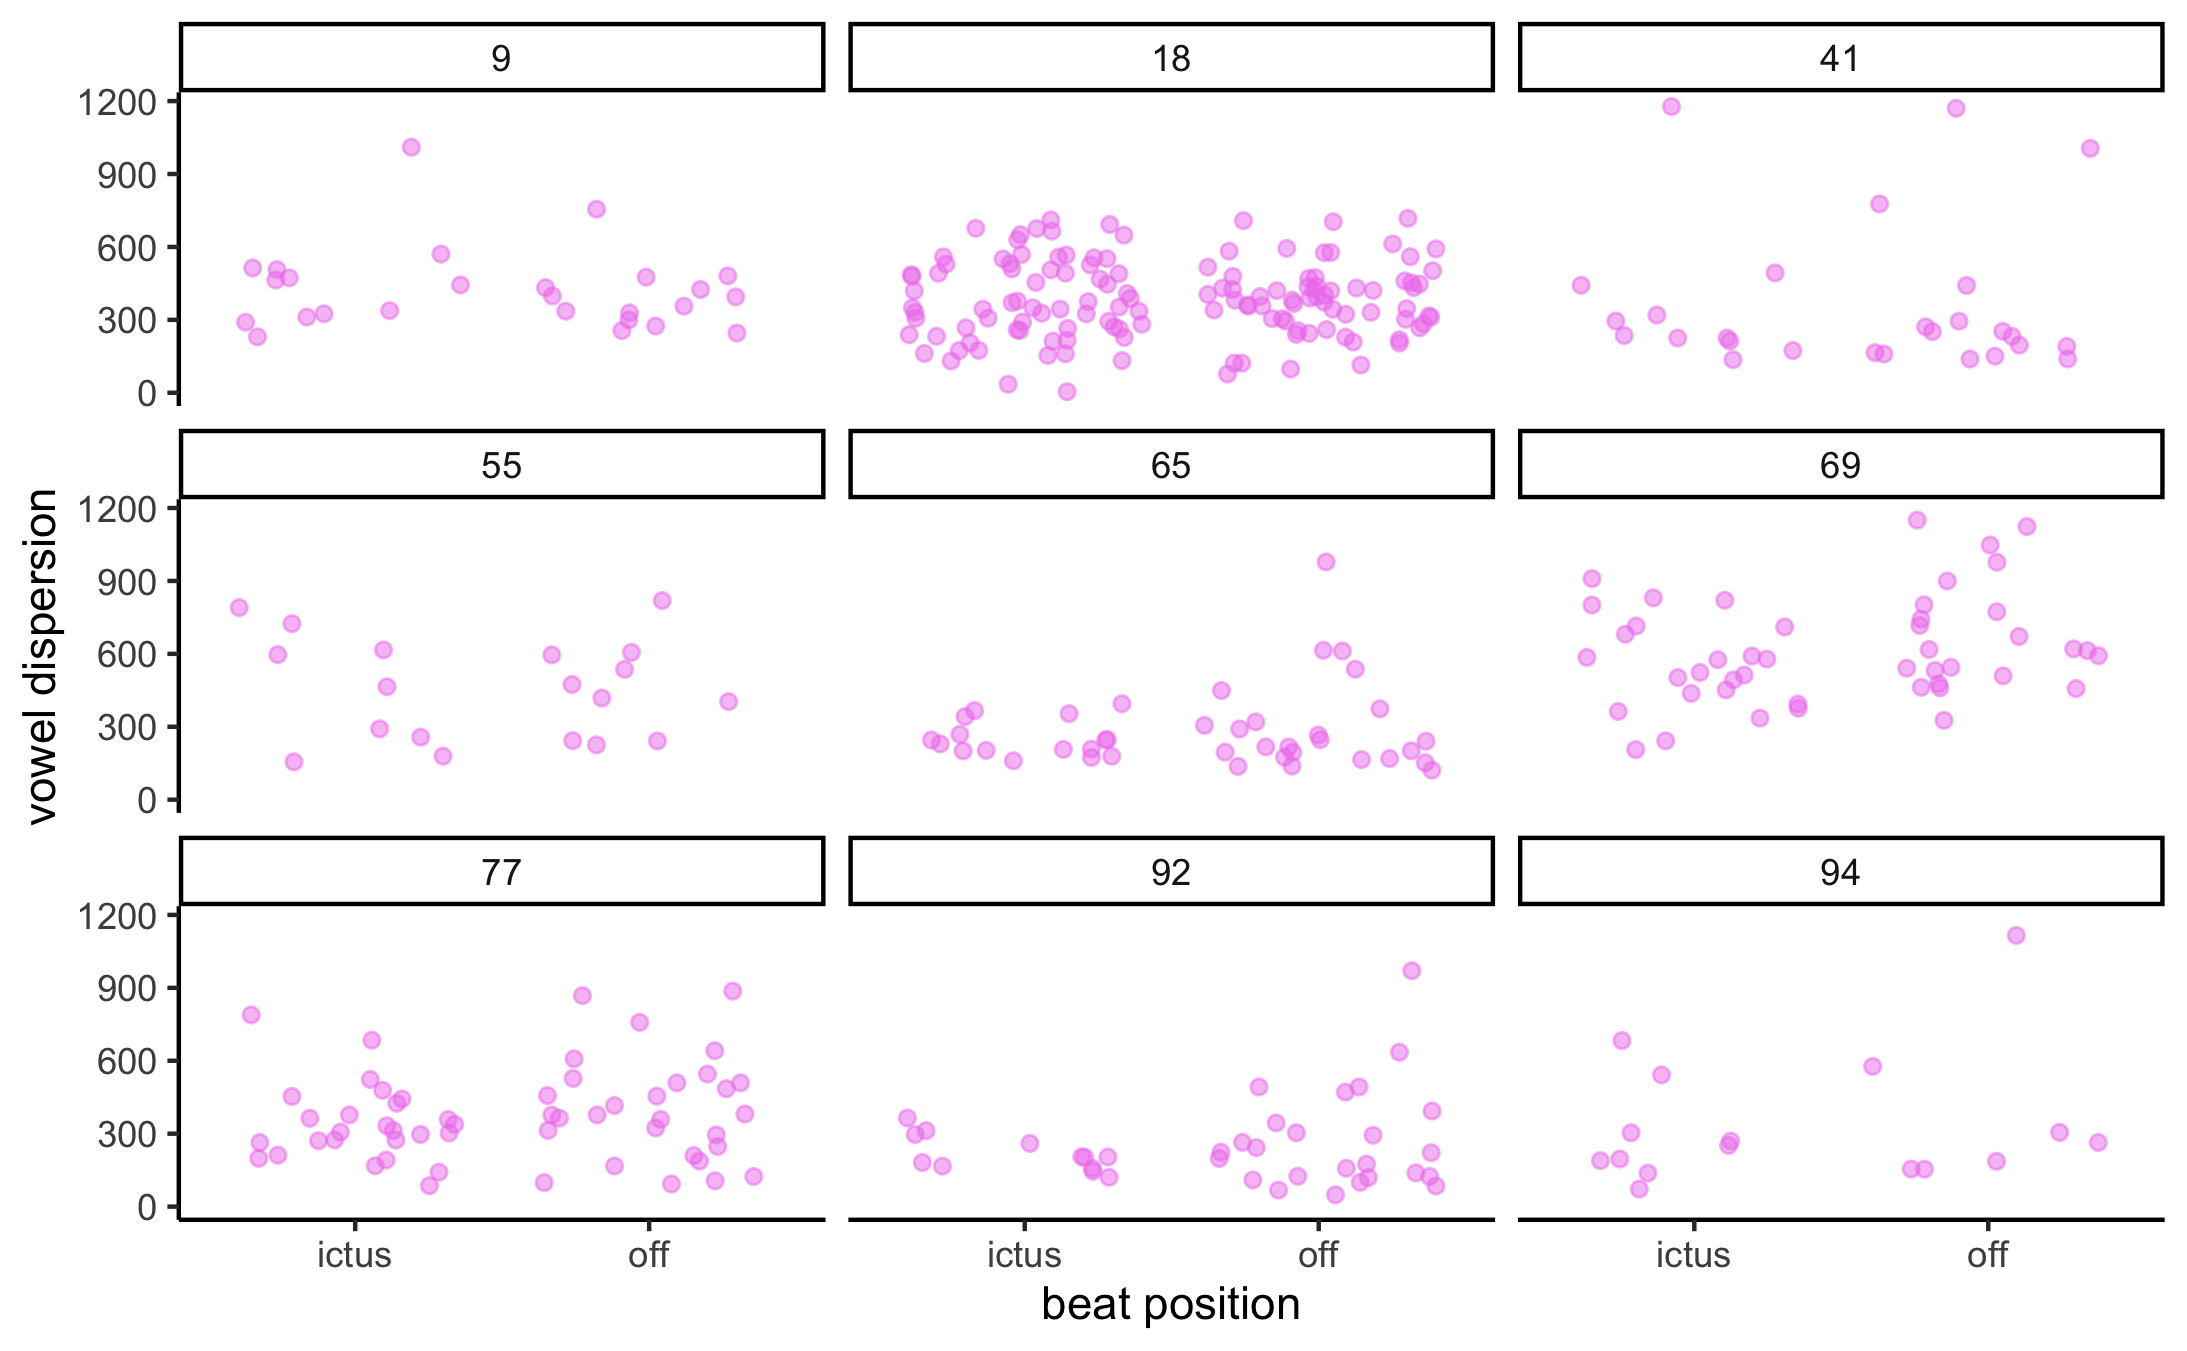
\includegraphics[width=\textwidth]{/Users/sarah/Git/regilaul_project/manuscript/results/song_euc_ictus.png}
\caption{euclidean distance of vowels on and off the beat by song}
\label{eucicksong}

\end{figure}